\begin{wrapfigure}[0]{r}[-1cm]{4cm}
 \vspace{-6cm}
  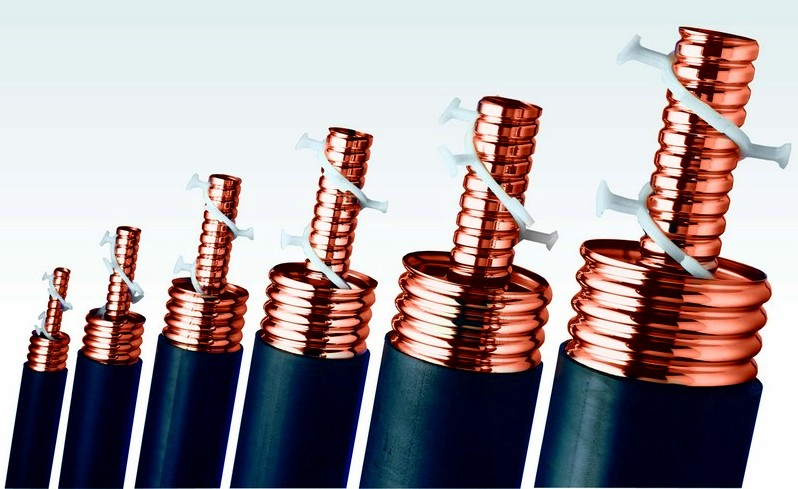
\includegraphics[scale=0.2]{DDK/Bilder/Cables.jpg}
 \vspace{-6cm}
\end{wrapfigure}

\section*{Theorie- und Prüfungsfragen}

~~~~~~
\subsection*{Die Dämpfung}

\begin{enumerate} 
\itemsep1pt\parskip0pt\parsep0pt
\item[1] Was wird unter dem Ausdruck Dämpfungsfaktor verstanden?
\loesung{Das Verhältnis von der am Anfang einer Übertragungsstrecke vorhandenen Leistung $P_1$ zu der am Ende übrig gebliebenen Leistung $P_2$ wird als Dämpfungsfaktor $D$ bezeichnet. $D_P = \dfrac{P_1}{P_2}$ }
\item[2] Was wird unter dem Ausdruck Verstärkungsfaktor verstanden?
\loesung{Das Verhältnis von der am Ende einer Übertragungsstrecke erreichten Leistung $P_2$ zu der am Eingang vorhandenen Leistung $P_1$ wird als Verstärkungsfaktor $T$ bezeichnet. $T = \dfrac{P_2}{P_1}$ }
\item[3] Zur besseren Handhabung ist es möglich die Dämpfung und die Verstärkung in $dB$ anzugeben. Wie lässt sich das berechnen?
\loesung{$a_p = 10 \cdot lg \dfrac{P_1}{P_2}$; $g=10 \cdot lg \dfrac{P_2}{P_1} $}
\item[4] Am Eingang bzw. am Ausgang einer Übertragungsstrecke liegen verschiedene Leistungen an. Berechne jeweils die fehlenden Einträge.
\end{enumerate}

\begin{figure}[H]
	\subfigure{
		\begin{tabular}{|l|l|l|l|}
			\hline
			Eingang & Ausgang & Dämpfung & Verstärkung\\
			\hline
			$1W$ & $4W$ &  & ~\hspace*{1cm}\\
			$4W$ & $1W$ &  & ~\hspace*{1cm}\\
			$4W$ & $10W$ &  & ~\hspace*{1cm}\\
			$50W$ &  & $-7dB$ & $7dB$\\
			\hline
		\end{tabular}
	}
	\subfigure{
		\loesung{
			\begin{tabular}{|l|l|l|l|}
				\hline
				Eingang & Ausgang & Dämpfung & Verstärkung\\
				\hline
				$1W$ & $4W$ &  & ~\hspace*{1cm}\\
				$4W$ & $1W$ &  & ~\hspace*{1cm}\\
				$4W$ & $10W$ &  & ~\hspace*{1cm}\\
				$50W$ &  & $-7dB$ & $7dB$\\
				\hline
			\end{tabular}
			}
	}
\end{figure}


\begin{enumerate} 
\itemsep1pt\parskip0pt\parsep0pt
\item[1] \emph{\textbf{TI}}  ...
	\begin{enumerate}
	\itemsep1pt\parskip0pt\parsep0pt
		\item[A] geht nicht über den geografischen Horizont hinaus. Sie wird in höheren Frequenzbereichen stärker gedämpft als in niedrigeren Frequenzbereichen.
		\item[B] geht über den geografischen Horizont hinaus. Sie wird in niedrigeren Frequenzbereichen stärker gedämpft als in höheren Frequenzbereichen.
		\item[C] geht über den geografischen Horizont hinaus. Sie wird in höheren Frequenzbereichen stärker gedämpft als in niedrigeren Frequenzbereichen.
		\item[D] geht nicht über den geografischen Horizont hinaus. Sie wird in niedrigeren Frequenzbereichen stärker gedämpft als in höheren Frequenzbereichen.
		\loesung{Lösung C}
	\end{enumerate}
\end{enumerate}